\documentclass[a4paper,10pt]{article}
\usepackage{fullpage}
\usepackage{graphicx}
\usepackage{amsmath}
\usepackage{url}
\usepackage{syntax}
\usepackage{listings}
\begin{document}

\title{Inducing Probabilistic Programs by Bayesian Program Merging}
\date{}
\maketitle
\begin{abstract}
This report outlines an approach for representing generative models with probabilistic programs and learning these programs from data.  The main advantage of using probabilistic programs as generative models is the ability to capture interesting patterns in a concise manner that is amenable to inference.  Formulating model learning in terms of program induction also leads us to explore the idea of understanding pattern as repeated computation within a generative model.  This idea provides a unifying theme for the program transformations used in searching the space of generative models, which is framed in a Bayesian model merging-like way.  There are two main types of program transformations we consider: the first is based on merging common subexpressions within a program and the second focuses on reducing the number of parameters for functions in the program.  We demonstrate this approach on a simple domain of colored trees.
\end{abstract}
\section{Introduction}
What do you see when you look at figure \ref{fig:plants}? What kinds of patterns are there in the image? 
\begin{figure}[h]
\begin{center}
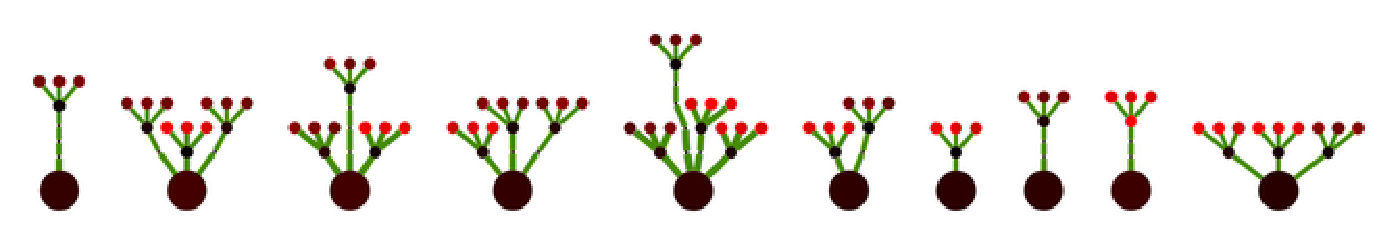
\includegraphics[scale=.60]{plants.pdf}
\end{center}
\label{fig:plants}
\caption{Some plants.}
\end{figure}

You might describe the image as a series of trees where each tree has a large base and a number of branches of variable length with each branch ending in a flower that is either light or dark red.  Each part of this description corresponds to a different pattern detected in the image.  The large base for each indiviual plant, the variable length branches, branches end in red flowers, etc.  Recognizing patterns like these is an important aspect of intelligence and it would be useful if we could automate this process.  One possible way to approach this problem is in terms of learning generative models represented as probabilistic programs.  In this document, we build on the notion of representing patterns or concepts as probabilistic programs \cite{A.Stuhlmueller:2010:6d11a} and begin to explore a family of algorithms for learning such programs.

One of the major difficulties with identifying regularities in data is the many notions of what it means to be a pattern and how this can vary with the types of data being analyzed.   We propose approaching this problem by performing a ``reduction'' on pattern recognition problems, first transforming data (whatever its type) into some canonical form (an expression in a programming language) and then using the notion of pattern as repeated computation in the program.  The main components of our approach are as follows: representation of data in terms of algebraic data types, representation of patterns in data as probabilitic programs, guiding search through program space using a Bayesian posterior probability, and creating search moves based on detecting repeated computation.  The general algorithm can be summarized as 1) turn the data into a large program 2) identify repeated computation in the large program and extract these patterns by merging different parts of the program 3) determine which merge moves to apply based on the posterior probability distribution of the program given the data.  The probabilistic programs learned in such a manner can be understood as generative models and reasoning about such models can be formulated in terms of probabilistic inference.  We illustrate these ideas on list structured data.  

Generative models play a prominent role in modern machine learning and understanding different classes of models e.g. hidden Markov models, probabilistic context-free grammars, etc. have led to a wide variety of applications.  There is a trade-off between the variety of patterns a model class is able to capture and the feasability of learning models in that class \cite{Russell2003}.  Much of machine learning has focused on studying classes of models with limited expressiveness in order to develop tractable algorithms for modeling large data sets.  Our investigation takes a different approach and explores how learning might proceed in a very expressive class of models with a focus on identifying patterns from very small amounts of data.  

We examine a class of generative models that are represented as programs in a probabilistic programming language.  These programs can have parameterized functions and recursion, which allow for natural representation of ``long-range'' dependencies and recursive patterns.  We will frame searching this space of models in terms of Bayesian model merging \cite{Stolcke:1994:IPG:645515.658235} and demonstrate the class' ability to capture interesting patterns in the list data domain.

Data is generated from such a model by evaluating the program.  Another way to view it is each program represents some probability distribution and each 
evaluation of the program results in a sample from the distribution. We implement these programs in a subset of the probabilistic programming language Church [add citation goodman et al].  


\subsection{Bayesian Model Merging}
Bayesian model merging is a framework for searching through a space of generative models in order to find one that accurately generates the desired data.  The main idea is search program space through a series of merge transformations and to use the posterior $P(M|D)$ as a criteria for selecting transformations, here $M$ is the model and $D$ is the training data.  The method works by creating an initial model that has a uniform distribution over the training set by explicitly incorporating each training point into the model (details are model class specific), this process is called data incorporation.  While the initial model has a good likelihood $P(D|M)$, it will never generate points outside the training set, in other words it severely overfits the initial data.  Alternative model hypotheses are explored by transforming the initial model with merge operations.  Merge operations collapse the structure of a model (again specific details are dependent on the model class) and the result may have better generalization properties.  This technique has been successfully applied to learning artificial probabilistic grammars where the grammars were represented as hidden Markov models, n-grams, and probabilistic context-free grammars.  Our work also uses the posterior distribution as a search criteria and merging model structure to achieve generalization.  Our work differs in that we use a significantly richer model class of probabilistic programs.  This allows for more complex patterns to be represented as well allowing for more types of transformations that lead to interesting generalization of the model, which can be thought of as lossy compression.   The use of programs as generative models also lends itself to a deeper understanding of the relationship between pattern, computation, and intelligence.

\section{Overview}
The main parts of Bayesian program merging are as follows:
\begin{description}
\item[Data and Language] Data is represented in terms of some algebraic data type, which gives us a way to form initial programs using the type constructors.  Programs are written in a formal language that consists of type constructors and additional operators.
\item[Programs]  Distributions over data can be represented with probabilistic programs and the structure of the programs corresponds to regularities in the data.
\item[Search] Search is based on identifying programs with a high posterior probability and then applying transformations to those programs to continue exploration.
\item[Merge Operations] Transformations on programs merge program structure, which can increase generalization of the model as well as the prior probability.
\end{description}
\section{Data Representation, Algebraic Data Types, and Language}
We assume the data we deal with can be modeled with an algebraic data type whose constructors are known to us.  This assumption gives us a starting point for program induction since any data can be directly translated into a program which is a derivation (sequence of constructor operations) of the data from the type specification. 
\subsection{Lists Example}
Looking back to figure \ref{fig:plants} we can model the trees in terms of lists or s-expressions.  Each tree consists of nodes, where each node has a size and color along with a list of child nodes.  This follows the classic recursive definition of a list below.   
\begin{grammar}
<tree> ::= '(node' <data> <tree> <tree> ... ')'

<data> ::= '(data' <color> <size> ')'

<color> ::= '(color' [number] ')'

<size> ::= '(size' [number] ')'
\end{grammar}
The following is an example of a tree expression along with a graphical representation.
\lstset{basicstyle=\small\ttfamily, frameround=fttt, breaklines=true, language=Lisp}
\begin{lstlisting}[mathescape=true]
(node (data (color (gaussian 50 25)) (size 1))
  (node (data (color (gaussian 30 25)) (size 0.3))
    (node (data (color (gaussian 225 25)) (size 0.3)))
    (node (data (color (gaussian 225 25)) (size 0.3)))
    (node (data (color (gaussian 225 25)) (size 0.3)))))
 $
\includegraphics[scale=1.0]{plant.pdf}$ 
\end{lstlisting}

We now have a way of representing data as rudimentary programs.  In order to capture interesting patterns we need a more expressive language.  We use the following subset of Church.  The grammar below lists language constructs available for Bayesian program merging in the tree domain:
\begin{grammar}
<expr> ::= '(begin ' <expr> <expr> ... ')' 
\alt <lambda expr> 
\alt <random expr>
\alt <func def>
\alt <func app>
\alt <var sym>
\alt [number]
\alt <tree>

<lambda expr> := '(lambda () ' <expr> ')'

<func def> ::= '(' define <func sym> <expr> ')'

<func app> ::= '(' <func sym> <expr> <expr> ... ')'
\alt '(' <lambda expr> <expr> ')'


<func sym> ::= 'F[number]' 
\alt list
\alt node
\alt data
\alt color
\alt size

<var sym> ::= 'V[number]'

<random expr> ::= '(uniform-draw (list' <expr> <expr> ... ')'
             \alt '(multinomial ' (list ' <expr> <expr> ... ') ('<expr> <expr> ...')' 
\end{grammar}

\subsection{Data Incorporation}
The first step of Bayesian program merging is data incorporation.  Data incorporation is the creation of an initial model by going through each example in the training set and creating an expression in terms of the algebraic data type constructors that evaluates to it.  These programs are combined into a single expression that draws uniformly over them.  In the case of the tree example we can define it as follows:
\begin{lstlisting}[frame=trBLsingle]
(define (incorporate-data data)
 (let* ([tree-expressions (map tree->expression data)])
  `(lambda () ((uniform-draw (list ,@(map thunkify tree-expressions)))))))

(define (thunkify sexpr) `(lambda () ,sexpr))
\end{lstlisting}
In the implementation the data or trees are s-expressions (an example being (((1) (2)))), which can be trivially converted into an expression in terms of the tree type constructors (the tree expression for the s-expression example is (node (data (color (gaussian 1 25)) (size 2)))).  For sake of expository simplicity we assume data is already a tree expression.  An important question we leave for future work is how to perform data incorporation when the data is less structured e.g. feature vectors.  If we give \texttt{incorporate-data} the input: 
\begin{lstlisting}[mathescape=true]
((node (data (color (gaussian 70 25)) (size 1))
             (node (data (color (gaussian 37 25)) (size 0.3))
               (node (data (color (gaussian 213 25)) (size 0.3)))
               (node (data (color (gaussian 207 25)) (size 0.3)))
               (node (data (color (gaussian 211 25)) (size 0.3)))))
(node (data (color (gaussian 43 25)) (size 1))
             (node (data (color (gaussian 47 25)) (size 0.1))
               (node (data (color (gaussian 33 25)) (size 0.3))
                 (node (data (color (gaussian 220 25)) (size 0.3)))
                 (node (data (color (gaussian 224 25)) (size 0.3)))
                 (node (data (color (gaussian 207 25)) (size 0.3)))))))
$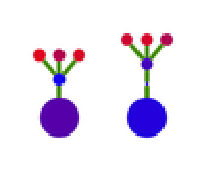
\includegraphics[scale=.7]{initData.pdf}$
\end{lstlisting}

We get the program 
\begin{lstlisting}[mathescape=true]
  (lambda ()
   ((uniform-draw
    (list
     (lambda ()
      (node (data (color (gaussian 70 25)) (size 1))
       (node (data (color (gaussian 37 25)) (size 0.3))
        (node (data (color (gaussian 213 25)) (size 0.3)))
        (node (data (color (gaussian 207 25)) (size 0.3)))
        (node (data (color (gaussian 211 25)) (size 0.3))))))
     (lambda ()
      (node (data (color (gaussian 43 25)) (size 1))
       (node (data (color (gaussian 47 25)) (size 0.1))
        (node (data (color (gaussian 33 25)) (size 0.3))
        (node (data (color (gaussian 220 25)) (size 0.3)))
        (node (data (color (gaussian 224 25)) (size 0.3)))
        (node (data (color (gaussian 207 25)) (size 0.3)))))))))))
$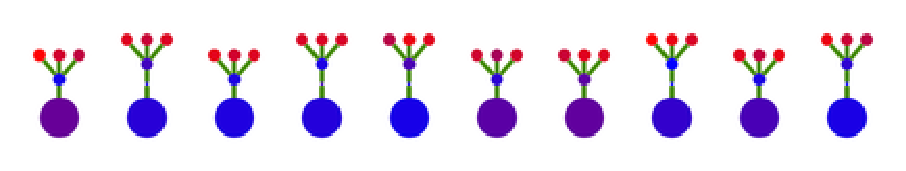
\includegraphics[scale=.7]{initProgram.pdf}$
\end{lstlisting}

\section{Probabilistic Programs}
A generative model is a probability distribution over data.  We can represent probability distributions as programs in a probabilistic programming language like Church \cite{N.D.Goodman:2008:f2a0d}.  One reason this is interesting is the structure of a program (i.e. the decomposition into functions and the flow of control) can capture different regularties in the data.    We illustrate this idea by looking at a probabilistic program that generates the images in figure \ref{fig:plants} and see how different parts of the program correspond to the different patterns we described earlier (functions and variables are given semantically meaningful names for readibility, but can easily be replaced by F[number] and V[number] to fit the grammar specified earlier).  
\begin{lstlisting}[mathescape=true]
(define tree
 (lambda ()
  (uniform-draw 
   (list
   (node (body) (branch)) 
   (node (body) (branch) (branch)) 
   (node (body) (branch) (branch) (branch))
   (node (body) (branch) (branch) (branch) (branch))))))

(define (body) 
 (data (color (gaussian 50 25)) (size 1)))

(define (branch)
 (multinomial (list (flower 150) (flower 255) (node (branch-info) (branch))) (list .25 .25 .50))) 

(define (branch-info)
 (data (color (gaussian 0 25)) (size .1)))

(define (flower shade)
 (node (data (color (gaussian 0 25)) (size .3))
  (petal shade)
  (petal shade)
  (petal shade)))

(define (petal shade)
 (node (data (color shade) (size .3))))
$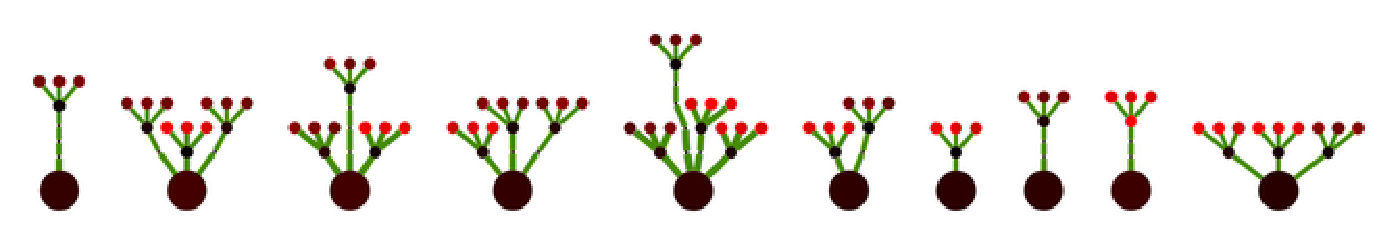
\includegraphics[scale=.25]{plants.pdf}$
\end{lstlisting}
We can think programs as a combination of data constructor operations with some additional control flow operations and lambda abstractions.  The program in figure \ref{prog:genModel} begins by determining the number of branches the tree will have and then creating a large body node that connects these branches.  Each branch function recursively connects a series of small nodes together and ends in a call to the flower function, passing it one of two colors.  The flower function creates a node with three ``petal'' nodes each of the same color.  Looking at this program we see how patterns such as a flower having three petals and the body having a large base are reflected in the program structure.  The compositionality of the language also captures relational patterns such as branches end in flowers.  Now that we know many different patterns can be represented within a probabilistic program, the main question becomes how do we change the structure of our initial data incorporated program to reflect such patterns.



\section{Bayesian Search}
The search over program space uses beam search as a guiding heuristic like in Bayesian model merging.  There is much that can be done in the way of employing this heuristic in complex search strategies, but for simplicity we use a straight-forward beam search.  

\subsection{Data Abstractions}
We use data abstractions for programs and functions created by merge operations on programs.  A function created by a merge operation is called an abstraction (after lambda abstraction).  It consists of a name, variables, and a pattern i.e. the s-expression that makes up the body of the function.  
\begin{lstlisting}[frame=trBL]
(define (make-abstraction pattern variables)
 (make-named-abstraction (sym FUNC-SYMBOL) pattern variables))
(define (make-named-abstraction name pattern variables)
 (list 'abstraction name variables pattern))

(define abstraction->name second)
(define abstraction->vars third)
(define abstraction->pattern fourth)
\end{lstlisting}
Here \texttt{sym} is used to create unique symbols in an orderly manner for use as function or variable names.


Programs represent the generative models we search over.  They consist of a list of abstractions and a body.
\begin{lstlisting}[frame=trBL]
(define (make-program abstractions body)
 (list 'program abstractions body))
(define program->abstractions second)
 (define program->body third)
\end{lstlisting}  

We use a wrapper around the programs to keep track of additional program information during search.  The motivation for this additional information will become clearer after reading the next section on beam search, but the basic idea is if a program's semantics are preserved after a transformation, the likelihood does not need to be recomputed (an expensive computation). The additional information in the wrapper is bookkeeping used to exploit this fact during search.  
\begin{lstlisting}[frame=trBL]
(define (make-program+ program posterior log-likelihood log-prior semantics-preserved)
 (list 'program+ program posterior log-likelihood log-prior semantics-preserved))
(define program+->program second)
(define program+->posterior third)
(define program+->log-likelihood fourth)
(define program+->log-prior fifth)
(define program+->semantics-preserved sixth)
(define (program+->program-transform semantics-preserved program+ new-program)
 (make-program+ new-program 
                (program+->posterior program+) 
                (program+->log-likelihood program+) 
                (program+->log-prior program+) 
                semantics-preserved))
\end{lstlisting}


\subsection{Beam Search}
We use a basic beam search to explore the space of generative models.  The posterior is used as the heuristic function in guiding search.
\begin{lstlisting}[frame=trBL]
(define (beam-search data init-program beam-size depth)
  (let* ([top-transformations 
          (sort-by-posterior
           data 
           (beam-search-transformations data init-program beam-size depth))]
         [da (display-all  "top transformations" top-transformations)])
    (if (null? top-transformations)
        init-program
        (program+->program (first top-transformations)))))

(define (beam-search-transformations data program beam-size depth)
  (let ([init-program+ (make-program+ program 0 0 0 #f)])
    (depth-iterated-transformations (lambda (programs+) 
                                     (best-n data programs+ beam-size)) 
                                    init-program+ depth)))

(define (best-n data programs n)
  (max-take (sort-by-posterior data programs) n))
\end{lstlisting}
The main part of the search is performed by \texttt{depth-iterated-transformations}, which recursively applies program transformations to the best programs at a given search depth and then filters the results to get the best programs for the next depth.
\begin{lstlisting}[frame=trBL]
(define (depth-iterated-transformations cfilter program+ depth)
  (let* ([da (display-all "CURRENT DEPTH: " depth)]
         [transformed-programs+ (apply-and-filter-transformations depth cfilter program+)])
    (delete '()  (append transformed-programs+
             (apply append (map (lambda (prog) 
                                 (depth-iterated-transformations cfilter prog (- depth 1))) 
                                transformed-programs+))))))
\end{lstlisting}
We reduce the amount of computation required when choosing the best programs at each level of search by separating program transformations that preserve semantics from those that do not.  Marking programs based on their transformation type allows us to reuse likelihood for a program that was created by a semantics preserving transformation.
\begin{lstlisting}[frame=trBL]
(define (apply-and-filter-transformations depth cfilter program+)
 (if (= depth 0)
     '()
     (let* ([semantics-preserved-programs+ (apply-transformations 
                                             program+ 
                                             semantic-preserving-transformations 
                                             #t)]
            [semantics-changed-programs+ (apply-transformations 
                                           program+ 
                                           semantic-changing-transformations 
                                           #f)])
       (cfilter (append semantics-preserved-programs+ semantics-changed-programs+)))))

(define (apply-transformations program+ transformations semantics-preserving)
  (let* ([program (program+->program program+)]
         [transformed-programs (delete '() 
                                 (concatenate 
                                   (map (lambda (transform) 
                                         (transform program #t)) 
                                        transformations)))]
         [transformed-programs+ (map (lambda (program) 
                                      (program+->program-transform 
                                        semantics-preserving 
                                        program+ 
                                        program)) 
                                     transformed-programs)])
    transformed-programs+))
\end{lstlisting}
The posterior distribution is estimated by combining an estimate of the likelihood with the computation of the prior.  
\begin{lstlisting}[frame=trBL]
(define (sort-by-posterior data programs+)
  (let* ([programs (map program+->program programs+)]
         [semantics-flags (map program+->semantics-preserved programs+)]
         [log-priors (map log-prior programs)]
         [da (display-all "log-priors: " log-priors "\n")]
         [log-likelihoods (map (lambda (prog+ semantics-flag)
                                 (if semantics-flag
                                     (program+->log-likelihood prog+)
                                     (log-likelihood data (program+->program prog+) 10))) 
                               programs+ 
                               semantics-flags)]
         [da (display-all "log-likelihoods: " log-likelihoods "\n")]
         [posteriors (map + log-priors log-likelihoods)] 
         [new-programs+ (map make-program+ 
                          programs posteriors log-likelihoods log-priors semantics-flags)]
         [posteriors> (lambda (a b) (> (program+->posterior a) (program+->posterior b)))])
    (list-sort posteriors> new-programs+)))
\end{lstlisting}
We use a prior based on program length like in Bayesian model merging.  
\begin{equation}P(M)\propto e^{-size(M)}\end{equation}
\begin{lstlisting}[frame=trBL]
(define (log-prior program)
  (- (program-size program)))
\end{lstlisting}
This prior effectively biases the search towards smaller programs.  A program's size is the number of symbols in the function bodies as well as the main body.
\begin{lstlisting}[frame=trBL]
(define (program-size program)
 (define (sexpr-size sexpr)
  (if (list? sexpr)
   (apply + (map sexpr-size sexpr))
   1))
 (define (abstraction-size abstraction)
  (sexpr-size (abstraction->pattern abstraction)))
 (let* ([abstraction-sizes (apply + (map abstraction-size (program->abstractions program)))]
        [body-size (sexpr-size (program->body program))])
  (+ abstraction-sizes body-size)))
\end{lstlisting}
The computation of the likelihood is the difficult part in estimating the posterior.  Intuitively we can think of it as way to say how good a particular program is at producing a set of target data.  This is important in search because it can give information on whether and/or how to adjust our hypothesis.  In a deterministic setting where the programs do not have randomness we can often have an intuitive sense of whether a program is good or bad based on some metric we make up on the output and the data.  Working in the probabilistic setting allows us to have a more standard way of deciding whether a program is good or bad.  The main idea being a probabilistic program is a generative process and represents a distribution over possible data.  Given the ``right'' random choices during the execution of the program the output will be the observed data.  By knowing the probabilities of these choices, we can combine them based on the rules of probability to get a score for how likely our program is to generate the observed data and this gives us a sense of whether the program is good or bad.  There may be many possible settings for the random choices of a program and this can make determining which choices lead to the observed data difficult.  There is an additional difficulty in that there could be many possible settings that lead to the observed data and we need to take take all of them into account.  We give an example of one possible way to approximate this computation for list-type data in the example below.
\subsubsection{Estimating Likelihood for List Programs}
The method used here is described for the sake of completeness, but it is not critical to the idea of Bayesian program merging and there are many ways computation of likelihood could be improved.  In the case of programs that generate list structured data we can estimate the likelihood by splitting the data into the discrete topology of the list and its continuous items.  This factors the problem in the following way:
\begin{eqnarray}
P(ls|p) &=& \prod_{ls}P(l|p)
\end{eqnarray}
where $ls$ stands for lists, our target data, the $l$ stands for a single list, and $p$ is the program.
\begin{lstlisting}[frame=trBL]
(define (log-likelihood lists-data prog sample-size)
  (apply + (map (lambda (single-list) 
                 (single-log-likelihood prog sample-size single-list)) 
                lists-data)))
\end{lstlisting}
The idea behind estimating the likelihood for a single tree, $P(l|p)$, is to evaluate the program several times forcing the computation to result in the target tree each time.  Each evaluation gives a probability for a possible way of generating the tree from the model.  This probability is the product of random choices made in the program during evaluation.  Since there may be several possible ways to generate the tree from the program we average the different evaluations.  In the code below \texttt{smc-core} (where smc stands for sequential Monte Carlo) is the part that forces evaluation of the program to the desired data.  A detailed description of \texttt{smc-core} is beyond the scope of this report, but it can be thought of as an incremental forward sampling process.  Due to the forward-sampling nature of this process, we separate random choices used in generating the continuous-valued parts of the tree (i.e. the color) from the random choices that influence the tree structure.
\begin{lstlisting}[frame=trBL]
(define single-log-likelihood 
   (lambda (program popsize tree)
     (let* ([new-program (replace-color program)]
            [model (eval (program->sexpr new-program))]
            [topology-scores+tree-parameters (compute-topology-scores+evaluate 
                                                model tree popsize)]
            [topology-scores (first topology-scores+tree-parameters)]
            [trees-with-parameters (second topology-scores+tree-parameters)]
            [color-scores (map (lambda (tree-with-parameters) 
                                 (compute-color-score tree tree-with-parameters)) 
                               trees-with-parameters)]
            [scores (map + topology-scores color-scores)]
            [score (if (null? scores)
                        -inf.0
                        (apply log-sum-exp scores))])
       score)))
\end{lstlisting}
We take advantage of fact that color is drawn from a Gaussian to compute the probability of observed color values.  We do this by modifying the color function to output the mean and variance for a particular node rather than a value drawn from a gaussian with these parameters.
\begin{lstlisting}[frame=trBL]
(define (replace-color program)
 (define (color? sexpr)
  (tagged-list? sexpr 'color))
 (define (return-parameters sexpr)
  `(list ,(second sexpr) 15))
 (define (replace-in-abstraction abstraction)
  (make-named-abstraction (abstraction->name abstraction) 
                          (sexp-search color? return-parameters (abstraction->pattern abstraction)) 
                          (abstraction->vars abstraction)))
 (let* ([converted-abstractions (map replace-in-abstraction (program->abstractions program))]
        [converted-body (sexp-search color? return-parameters (program->body program))])
  (make-program converted-abstractions converted-body)))
\end{lstlisting}
The modfied program is evaluated several times to generate trees whose topology (node structure) matches the observed tree and has the parameters for the Gaussian used to generate a color.  During the evaluation of the modified program we also capture the probability for the choices made in generating the topology of the tree.  The references to laziness are related to the implmentation of the sequential Monte Carlo procedure and the details are not critical to the report.
\begin{lstlisting}[frame=trBL]
(define (compute-topology-scores+evaluate model tree popsize)
  (let* ([lazified-tree (list->lazy-list tree)]
         [samples (smc-core 
                   (map list (iota (+ 1 (lazy-list-size  lazified-tree)))) popsize 20
                     (lambda (depth) (lambda () (let ((s (model)))
                      (pair (lazy-topology-equal? s lazified-tree depth)
                       (lambda () (first (lazy-list->list s depth))))))))]
         [samples (fold (lambda (s a) 
                         (if (member (mcmc-state->addrval s) 
                           (map (lambda (x) (mcmc-state->addrval x repeat-symbol)) a)) 
                           a (pair s a))) '() samples)]
         [topology-scores (map mcmc-state->score samples)]
         [generated-trees (map mcmc-state->query-value samples)])
    (list topology-scores generated-trees)))
\end{lstlisting}
We can use the Gaussian parameters for each node's color to determine the probability of the observed color values of a tree.
\begin{lstlisting}[frame=trBL]
(define (compute-color-score tree tree-with-parameters)
 (if (null? tree)
  0
 (+ (single-color-score (node->color tree) (node->color tree-with-parameters)) 
    (apply + (map compute-color-score 
                 (node->children tree) 
                 (node->children tree-with-parameters))))))

(define (single-color-score x mean+variance)
  (log (normal-pdf (first x) (first mean+variance) (second mean+variance))))
\end{lstlisting}
\section{Merge Operations}
We described earlier how patterns in the program representation of data can be viewed as repeated computation.  Here we describe how this idea manifests itself as specific program transformations used in exploring the search space.

\subsection{Inverse Inlining}
Inlining is the process of replacing function calls in a program with the body of the function called.  Inverse inlining creates new functions based on patterns in subexpressions of a program and replaces these subexpressions with functions calls for the new function.  We can think of this process as creating lambda abstractions that potentially compress the program by removing duplication in the code and acts as a proxy for reconizing repeated computation.  The following code fragment outlines this procedure where compressions finds the different (lambda) abstractions that can be formed by anti-unifying (partially matching) pairs of subexpressions in a condensed form of the program (only the bodies of the functions and the body of the program).  Duplicate abstractions are filtered out then potential program transformations are created by inverse-inlining function calls for each of the abstractions.  

\begin{lstlisting}[frame=trBL]
(define (compressions program . nofilter)
 (let* 
  ([condensed-program (condense-program program)]
   [abstractions (possible-abstractions condensed-program)]
   [compressed-programs (map (curry compress-program program) abstractions)]
   [program-size (size (program->sexpr program))]
   [valid-compressed-programs
    ...find the compressed-programs smaller than the original program
    if nofilter is present then all compressed-programs are returned
   ])
 valid-compressed-programs))

(define (condense-program program)
 `(,@(map abstraction->pattern (program->abstractions program))
  ,(program->body program)))

(define (possible-abstractions expr)
 (let* 
  ([subexpr-pairs (list-unique-commutative-pairs (all-subexprs expr))]
   [abstractions (map-apply (curry anti-unify-abstraction expr) subexpr-pairs)])
  (filter-abstractions  abstractions)))
\end{lstlisting}

Aside from the obvious correspondence between repetition in program syntax and repetition in computation, there are a few different reasons for believing this is a useful program transformation.  In terms of Bayesian model merging we are merging the structure of the model, which potentially leads to models with better generalization properties \cite{Stolcke:1994:IPG:645515.658235}.  Inverse-inlining can also also be interpreted as doing something similar to finding partial symmetries in inverse-procedural modeling \cite{DBLP:journals/tog/BokelohWS10}, which was successful in capturing the patterns of various 3-d models.

\subsubsection{Overview}
The following example illustrates the inverse inlining transformation
\begin{lstlisting}[mathescape=true]
(define (inverse-inlining-example)
 (uniform-draw 
   (node
     (node a (node a (node b) (node b)))
     (node a (node a (node c) (node c))))))
$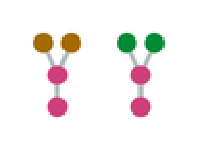
\includegraphics[scale=.40]{csrExample.pdf}$
\end{lstlisting}
a possible result of this transformation would be
\begin{lstlisting}[mathescape=true]
(begin
  (define (F1 V1 V2)
    (node a (node a (node V1) (node V2))))
  (uniform-draw (node (F1 b b) (F1 c c))))

$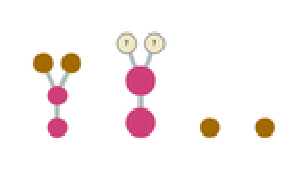
\includegraphics[scale=.40]{csrDecompose1.pdf}\\
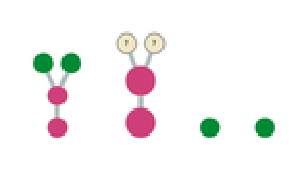
\includegraphics[scale=.40]{csrDecompose2.pdf}$
\end{lstlisting}
The first thing to note is both programs have the same behavior, in that both return either \texttt{(a (a (b) (b)))} or \texttt{(a (a (c) (c)))} with equal probability.

  The transformation can be described as refactoring subexpressions that partially match in a program with a function whose body is the common parts of the matching subexpressions.  In the above example the subexpressions that partially match are \texttt{(node a (node a (node b) (node b)))} and \texttt{(node a (node a (node c) (node c)))}.  The common subexpression is \texttt{(node a (node a (node x) (node y)))}, the function created using this common subexpression is \texttt{F1} and the original subexpressions are refactored as \texttt{(F1 b b)} and \texttt{(F1 c c)}.

An inverse inlining transformation can be created for each pair of subexpressions that have a partial match.  In the case of \texttt{(+ (+ 2 2) (- 2 5))} the following pairs of subexpressions have a partial match: \texttt{[2,2], [(+ 2 2), (- 2 5)], [(+ 2 2), (+ (+ 2 2) (+ 2 5))], [(+ 2 5), (+ (+ 2 2) (+ 2 5))]}, the only subexpressions that do not have a partial match in this example.
\subsubsection{Anti-unification}
The process of finding a partial match between two expressions is called anti-unification.  One way to understand the process is in terms of the syntax trees for the expressions.  Every s-expression can be thought of as a tree where the lists and sublists of the s-expression make up the interior nodes and the primitive elements of the lists (e.g. symbols, numbers, etc.) are the leaves.  The tree in figure \ref{expressionTree} corresponds to the expression \texttt{(+ (+ 2 2) (- 2 5))}.  Finding a partial match between two expressions can be thought of as finding a common subtree between their tree representations.
\begin{figure}
\begin{center}
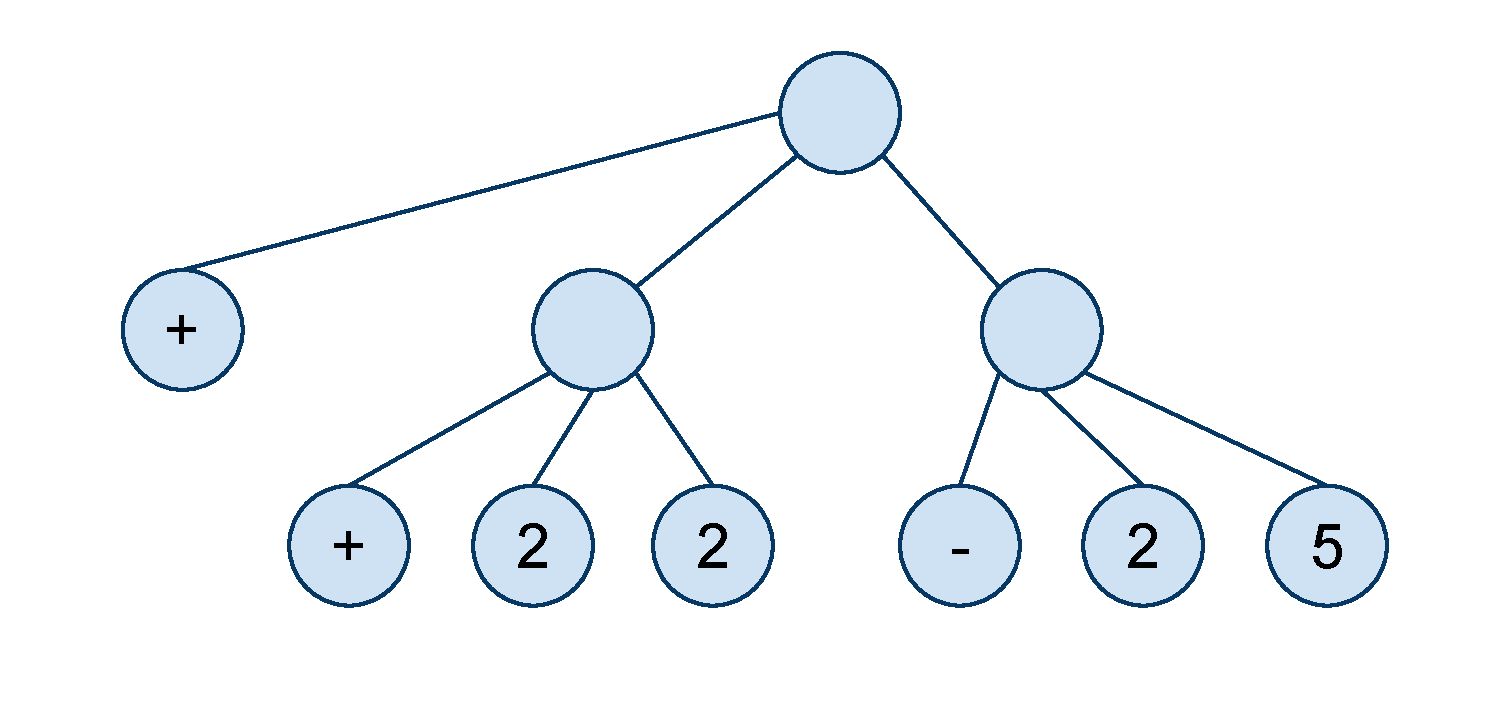
\includegraphics[scale=.40]{expressionTree.pdf}
\label{expressionTree}
\caption{An expression represented as a tree.}
\end{center}
\end{figure}

Anti-unification proceeds by recursively comparing two expressions, A and B (performed by \texttt{build-pattern}).  If A and B are the same primitive that primitive is returned.  If A and B are lists $(a_1,\ldots,a_n)$ and $(b_1,\ldots,b_n)$ of the same length then a list C $(c_1,\ldots,c_n)$ where each element $c_i$ is the anti-unification $a_i$ and $b_i$ is returned.  For all other cases when A and B do not match a variable is returned.

\begin{lstlisting}[frame=trBL]
(define anti-unify
 (lambda (expr1 expr2)
  (begin
   (define variables '())
   (define (add-variable!)
     (set! variables (pair (sym (var-symbol)) variables))
     (first variables))
   (let ([pattern (build-pattern expr1 expr2)])
    (list pattern (reverse variables))))))

(define (build-pattern expr1 expr2)
 (cond 
  [(and (primitive? expr1) (primitive? expr2)) (if (equal? expr1 expr2) expr1 (add-variable!))]
  [(or (primitive? expr1) (primitive? expr2)) (add-variable!)]
  [(not (eqv? (length expr1) (length expr2))) (add-variable!)]
  [else
   (let ([unified-expr 
         (map (lambda (subexpr1 subexpr2) (build-pattern subexpr1 subexpr2))
          expr1 expr2)])
     unified-expr)]))
\end{lstlisting}

\subsubsection{Anti-unification example}
We illustrate the process of anti-unification on the expressions \texttt{(+ (+ 2 2) (- 2 5))} and \texttt{(+ (- 2 3) 4)}
The first step is to compare the root of the trees and make sure we have lists of the same size, in this case they are both of size three so we have a matching roots and a partial match of \texttt{(* * *)} where the *'s are yet to be determined.
Now we recursively attempt to match the three subexpressions + with +, \texttt{(+ 2 2)} with \texttt{(- 2 3)}, and \texttt{(- 2 5)} with 4.
Since + and + are both primitives that are the same they match, and our partial match is now \texttt{(+ * *)}.
Comparing \texttt{(+ 2 2)} and \texttt{(- 2 3)} we see that they are both lists of size 3 and so they match giving us a total partial match of \texttt{(+ (* * *) *)}.
Again we recursively match subexpressions of \texttt{(+ 2 2)} and \texttt{(- 2 3)} i.e. + to -, 2 to 2, and 2 to 3.
Since + and - are primitives that don't match we replace them with a variable to get a total partial match of \texttt{(+ (V1 * *) *)}

Likewise after comparing 2 to 2 and 2 to 3 we'll get \texttt{(+ (V1 2 V2) *)} as our partial match.
In the final comparison of \texttt{(- 2 5)} and 4 we check can see there is no match because one \texttt{(- 2 5)} is a list and 4 is a primitive so the final result of our anti-unification is \texttt{(+ (V1 2 V2) V3)}.


\subsubsection{Compressing programs}
Now that we have created lambda abstractions from the partial matches between two subexpressions of some program, P, we can use these abstractions to compress P.  The idea will be to take the pattern of the abstraction and replace any subexpressions of P that fit the pattern.  A subexpression that fits the pattern is replaced by an application of the lambda abstraction.  We first do this replacement for each of the functions in P and then the body, resulting in a program P'.  After all the replacements are made, the lambda abstraction is inserted into the set of functions for P' and this is our refactored program.
\begin{lstlisting}[frame=trBL]
(define (compress-program program abstraction)
 (let* ([compressed-abstractions 
          (map (curry compress-abstraction abstraction)
               (program->abstractions program))]
        [compressed-body (replace-matches (program->body program) abstraction)])
  (make-program (pair abstraction compressed-abstractions) compressed-body)))
                           

(define (compress-abstraction compressor compressee)
 (make-named-abstraction (abstraction->name compressee)
                         (replace-matches (abstraction->pattern compressee) compressor)
                         (abstraction->vars compressee)))
\end{lstlisting}
Finding and replacing pattern matches of an abstraction F in an expression E proceeds recursively by taking the body of F and trying to match it to the expressio on E.  A match between the body of the abstraction and the expression is determined by unification, if a match exists then the application of F is returned where the arguments to F are refactored (if F has arguments).  If the match does not hold then E is returned with each of its subexpressions refactored.  If E is a primitive and not a match it is returned.

\begin{lstlisting}[frame=trBL]
(define (replace-matches s abstraction)
 (let ([unified-vars (unify s
                      (abstraction->pattern abstraction)
                      (abstraction->vars abstraction))])
  (if (false? unified-vars) ;;a function call for the abstraction is returned if there is a match
   (if (list? s)
    (map (lambda (si) (replace-matches si abstraction)) s)
    s)
   (pair (abstraction->name abstraction)  
         (map (lambda (var) (replace-matches (rest (assq var unified-vars)) abstraction))
          (abstraction->vars abstraction))))))
\end{lstlisting}
\subsubsection{Compressing Program Example}
In the case of \texttt{(+ (+ 2 2) (- 2 5))} the partial match we would get between the subexpression \texttt{[(+ (+ 2 2) (- 2 5)), (+ 2 2)]} is \texttt{(+ V1 V2)}.  We refactor the original expression \texttt{(+ (+ 2 2) (- 2 5))} in terms of \texttt{(+ V1 V2)} by creating a function \texttt{(define (F1 V1 V2) (+ V1 V2))} and applying it in the expression.  For example one application could be \texttt{(F1 (+ 2 2) (- 2 5))} and another could be \texttt{(+ (F1 2 2) (- 2 5))}.  In general we'll apply the function everywhere possible and get a refactored program like so...
\begin{lstlisting}
(+ (+ 2 2) (- 2 5))
=>
(begin
  (define (F1 V1 V2) (+ V1 V2))
  (F1 (F1 2 2) (- 2 5)))
\end{lstlisting}
The input to the refactoring procedure is a function, F, created from anti-unification and an expression, E, which will be refactored in terms of F.  In the example above F was \texttt{(define (F1 V1 V2) (+ V1 V2))}, E would be \texttt{(+ (+ 2 2) (- 2 5))}, and the result of refactoring was 
\begin{lstlisting}
(begin
  (define (F1 V1 V2) (+ V1 V2))
  (F1 (F1 2 2) (- 2 5))).
\end{lstlisting}

In the example \texttt{(+ (+ 2 2) (- 2 5))} matches \texttt{(+ V1 V2)} so an application of F1 to refactored arguments \texttt{(+ 2 2)} and \texttt{(- 2 5)} is returned resulting in \texttt{(F1 (F1 2 2) (- 2 5))}.  


\subsubsection{Unification}
Determining whether there is a match between a function body and an expression is known as unification.  Earlier we described anti-unification which can be thought of as a process to create a pattern from two expressions, unification can be viewed as the opposite process of seeing if and how a given pattern fits onto an expression.  The return value of unification is a list of assignments for the variables of the function that would make the function the same as the expression.

The input to unification is a function F, and an expression E.  Unification occurs recursively by checking whether the body of F and E are lists of the same size.  If they are the same size then unification returns the unification of each of the subexpressions.  If they are not the same size or only one of them is a list unification returns false.  In the case where both expressions being unified are primitives true is returned if they are equal and false otherwise.  In the case where the function expression of the unification is a variable an assignment is returned i.e. the variable along with the other expression passed to unification.  At the end a check is made to see if any unifications have returned false, in which case unification of F and E returns false.  There is also a check that any variable that is repeated in F has the same value assigned to it for each place it appears.  If this is not the case unification returns false. If unification is not false then an assignment for each unique variable of F is returned.

\begin{lstlisting}[frame=trBL]
(define unify
 (lambda (s sv vars)
  (cond [(variable? sv) (if (eq? s 'lambda) #f (list (pair sv s)))]
        [(and (primitive? s) (primitive? sv)) (if (eqv? s sv) '() #f)]
        [(or (primitive? s) (primitive? sv)) #f]
        [(not (eqv? (length s) (length sv))) #f]
        [else
         (let ([assignments (map (lambda (si sj) (unify si sj vars)) s sv)])
          (if (any false? assignments)
           #f
           (check/remove-repeated (apply append assignments))))])))

(define (variable? obj)
                 (member obj vars))

(define (check/remove-repeated unified-vars)
 (let* ([repeated-vars (filter more-than-one (map 
                        (curry all-assoc unified-vars) 
                        (map first unified-vars)))])
  (if (and (all (map all-equal? repeated-vars)) (not (any false? unified-vars)))
   (delete-duplicates unified-vars)
   #f)))
\end{lstlisting}
\subsubsection{Unification Example}
The example listed earlier where the function F is \texttt{(define (F1 V1 V2) (+ V1 V2))} and the s-expression being refactored is \texttt{(+ (+ 2 2) (- 2 5))} is used to illustrate unification.  Since \texttt{(+ (+ 2 2) (- 2 5))} and \texttt{(+ V1 V2)} are the same length unification is applied to the subexpression pairs \texttt{[+,+], [(+ 2 2), V1], [(- 2 5), V2]}.

Unification between + and + returns nothing since neither is a variable and they match.  Unification between \texttt{(+ 2 2)} and V1 returns the assignment of \texttt{(+ 2 2)} to V1 and likewise for \texttt{(- 2 5)} and V2.  So the function F1 matches the s-expression \texttt{(+ (+ 2 2) (- 2 5))} with variable assignments \texttt{V1:=(+ 2 2)} and \texttt{V2:=(- 2 5)}.

If the expression being unified with F1 had been \texttt{(- (+ 2 2) (- 2 5))} then unification between the outer - of the expression and the + of F1 would have returned false and the unification would have failed.

\subsubsection{Summary}
Inverse-inlining is a useful program transformation that identifies repeated computation in a program by finding patterns in its syntax.  These patterns in syntax correspond to patterns in the data.  We can understand this in terms of repeated computation as well in the sense that repeated syntax corresponds to repeated sequences of operations.  This might seem like a limited notion of pattern, but it is worth contemplating the role of lambda abstraction in the lambda calculus and the expressiveness of this language despite (or perhaps because of) its simplicity.

The process of inverse inlining follows two main steps 1) create abstractions from common subexpressions in a program via anti-unification 2) compress the program with the abstractions by replacing instances of the abstraction with a function application via unification.  Going back to our tree example we illustrate the process on the program in figure \ref{initProgram}.
A few of the abstractions found with anti-unification that create the smallest compressed programs are 
\begin{lstlisting}
((abstraction F1 (V1) (data (color V1) (size 0.3))))

((abstraction F1 (V1) (node (data (color V1) (size 0.3)))))

((abstraction F1 (V1 V2) (data (color V1) (size V2))))

((abstraction F1 (V1 V2 V3 V4 V5 V6)
       (node (data (color V1) (size V2))
         (node (data (color V3) (size 0.3))
           (node (data (color V4) (size 0.3)))
           (node (data (color V5) (size 0.3)))
           (node (data (color V6) (size 0.3)))))))

((abstraction F1 (V1 V2 V3 V4)
       (node (data (color V1) (size 0.3))
         (node (data (color V2) (size 0.3)))
         (node (data (color V3) (size 0.3)))
         (node (data (color V4) (size 0.3))))))
\end{lstlisting}
The following are the programs compressed using these abstractions.
\begin{lstlisting}
(begin
  (define F1 (lambda (V1) (data (color V1) (size 0.3))))
  ((uniform-draw
    (list
     (lambda ()
      (node (data (color (gaussian 70 25)) (size 1))
       (node (F1 37) 
         (node (F1 213)) (node (F1 207)) (node (F1 211)))))
     (lambda ()
      (node (data (color (gaussian 43 25)) (size 1))
       (node (data (color (gaussian 47 25)) (size 0.1))
        (node (F1 33) 
         (node (F1 220)) (node (F1 224)) (node (F1 207))))))))))

(begin
    (define F1
      (lambda (V1) (node (data (color V1) (size 0.3)))))
      ((uniform-draw
         (list
           (lambda ()
             (node (data (color (gaussian 70 25)) (size 1))
               (node (data (color (gaussian 37 25)) (size 0.3)) (F1 213)
                 (F1 207) (F1 211))))
           (lambda ()
             (node (data (color (gaussian 43 25)) (size 1))
               (node (data (color (gaussian 47 25)) (size 0.1))
                 (node (data (color (gaussian 33 25)) (size 0.3)) (F1 220)
                   (F1 224) (F1 207)))))))))

(begin
    (define F1 (lambda (V1 V2) (data (color V1) (size V2))))
      ((uniform-draw
         (list
           (lambda ()
             (node (F1 70 1)
               (node (F1 37 0.3) (node (F1 213 0.3))
                 (node (F1 207 0.3)) (node (F1 211 0.3)))))
           (lambda ()
             (node (F1 43 1)
               (node (F1 47 0.1)
                 (node (F1 33 0.3) (node (F1 220 0.3))
                   (node (F1 224 0.3)) (node (F1 207 0.3))))))))))
  (begin
    (define F1
      (lambda (V1 V2 V3 V4 V5 V6)
        (node (data (color V1) (size V2))
          (node (data (color V3) (size 0.3))
            (node (data (color V4) (size 0.3)))
            (node (data (color V5) (size 0.3)))
            (node (data (color V6) (size 0.3)))))))
      ((uniform-draw
         (list (lambda () (F1 70 1 37 213 207 211))
           (lambda ()
             (node (data (color (gaussian 43 25)) (size 1))
               (F1 47 0.1 33 220 224 207)))))))
  (begin
    (define F1
      (lambda (V1 V2 V3 V4)
        (node (data (color V1) (size 0.3))
          (node (data (color V2) (size 0.3)))
          (node (data (color V3) (size 0.3)))
          (node (data (color V4) (size 0.3))))))
      ((uniform-draw
         (list
           (lambda ()
             (node (data (color (gaussian 70 25)) (size 1))
               (F1 37 213 207 211)))
           (lambda ()
             (node (data (color (gaussian 43 25)) (size 1))
               (node (data (color (gaussian 47 25)) (size 0.1))
                 (F1 33 220 224 207)))))))))
\end{lstlisting}
The last abstraction captures the flower pattern we mentioned earlier.  Intuitively it seems like we can capture even more structure and replace the variables for the petal colors with a fixed value since they are all similar.  So rather than explaining the data as being drawn from several gaussians with slightly different means, we would like to say the data comes from only one gaussian with a single mean.  We address this issue in the next section with another type of program transformation.
\subsection{Deargument}
Deargument is a program transformation that takes a function in a program and removes one of its arguments.  The variable that is removed is redefined inside the function in terms of all the values it has been assigned (i.e. the values passed to the function for that variable during an application).  We can create different program transformations by allowing multiple schemes for redefining a variable, via \texttt{replacement-function},  as a function of its instantiations.  
\begin{lstlisting}[frame=trBL]
(define (deargument replacement-function program abstraction variable)
 (let* ([new-abstraction (remove-abstraction-variable 
                           replacement-function 
                           program abstraction 
                           variable)])
   (if (null? new-abstraction)
    '()
    (let* ([program-with-new-abstraction (program->replace-abstraction 
                                           program new-abstraction)]
           [new-program (remove-application-argument 
                          program-with-new-abstraction 
                          abstraction 
                          variable)])
      new-program))))
\end{lstlisting}
The abstraction whose variable is being removed keeps the same body, but the variable removed is now assigned a value  within the body instead of having its value passed in as an argument.
\begin{lstlisting}[frame=trBL]
(define (remove-abstraction-variable replacement-function program abstraction variable)
 (let* ([variable-instances (find-variable-instances program abstraction variable)]
        [variable-definition (replacement-function program abstraction variable variable-instances)])
   (if (equal? variable-definition NO-REPLACEMENT)
    '()
    (let* ([new-pattern 
            `((lambda (,variable) ,(abstraction->pattern abstraction)) ,variable-definition)]
           [new-variables (delete variable (abstraction->vars abstraction))])
     (make-named-abstraction (abstraction->name abstraction) new-pattern new-variables)))))

(define (program->abstraction-applications program target-abstraction)
 (define (target-abstraction-application? sexpr)
  (if (non-empty-list? sexpr)
   (if (equal? (first sexpr) (abstraction->name target-abstraction))
     #t
     #f)
   #f))
 (let* ([abstraction-patterns (map abstraction->pattern (program->abstractions program))]
        [possible-locations (pair (program->body program) abstraction-patterns)])
  (deep-find-all target-abstraction-application? possible-locations)))

(define (deep-find-all pred? sexp)
           (filter pred? (all-subexprs sexp)))

(define (all-subexprs t)
 (let loop ([t (list t)])
   (cond [(null? t) '()]
         [(primitive? (first t)) (loop (rest t))]
         [else (pair (first t) (loop (append (first t) (rest t))))])))

(define (find-variable-instances program abstraction variable)
 (let* ([abstraction-applications (program->abstraction-applications program abstraction)]
        [variable-position (abstraction->variable-position abstraction variable)]
        [variable-instances (map (curry ith-argument variable-position) abstraction-applications)])
   variable-instances))

(define (ith-argument i function-application)
           (list-ref function-application (+ i 1)))
\end{lstlisting}
After the abstraction has been adjusted, any place it was used (i.e. the function was applied) needs to be changed so that no values are passed in to the variable that was removed.
\begin{lstlisting}[frame=trBL]
(define (remove-application-argument program abstraction variable)
 (define (abstraction-application? sexpr)
  (if (non-empty-list? sexpr)
   (equal? (first sexpr) (abstraction->name abstraction))
   #f))
  (define (change-application variable-position application)
   (define (change-recursive-arguments argument) 
     (if (abstraction-application? argument)
       (change-application variable-position argument)
       argument))
   (let* ([ith-removed (remove-ith-argument variable-position application)])
    (map change-recursive-arguments ith-removed)))
 
  (remove-ith-argument variable-position application))
 (let* ([variable-position (abstraction->variable-position abstraction variable)]
        [program-sexpr (program->sexpr program)]
        [changed-sexpr 
         (sexp-search abstraction-application? 
                      (curry change-application variable-position) 
                      program-sexpr)]
        [new-program (sexpr->program changed-sexpr)])
   new-program))
  
(define (sexp-search pred? func sexp)
 (if (pred? sexp)
  (func sexp)
  (if (list? sexp)
   (map (curry sexp-search pred? func) sexp)
   sexp)))
\end{lstlisting}
This transformation is useful for generalizing a program to have recursive structure as well as dealing with continuous data types that may be distorted with noise, for example the color data of the tree examples.

\subsubsection{Noisy data example}
One issue with inverse-inlining is anything other than perfect equality results in the creation of a variable when matching two expressions.  So if we have an expression such as \texttt{(+ 2 2} and \texttt{(+ 2 2.01)} and we know there is some noise in the system then we may went to treat these expressions as if they were the same i.e. inverse inline them to \texttt{(define (F1) (+ 2 2)} or \texttt{(define (F1) (+ 2 2.01)} rather than \texttt{(define (F1 x) (+ 2 x)}.  We can do this using a deargument transformation along with a \texttt{replacment-function} called \texttt{noisy-number-replacment} that replaces the variable with the mean of its instances.  
\begin{lstlisting}[frame=trBL]
(define (noisy-number-replacement program abstraction variable variable-instances)
 (if (all (map number? variable-instances))
  (let* 
   ([instances-mean (mean variable-instances)])
    instances-mean)
  NO-REPLACEMENT))
\end{lstlisting}
One possible problem with this implmentation is we may end up creating many program transformations that will end up having a low likelihood because the variable instances do not actually come from the same gaussian.  Since the likelihood calculation is expensive we can try to avoid this by adding a test to see whether the numbers are close together.  If the numbers are close then the program is transformed otherwise it is not.  The down side is our definition of what is close is brittle and we may end up not transforming a program that should be transformed.
\begin{lstlisting}[frame=trBL]
(define (noisy-number-replacement program abstraction variable variable-instances)
 (define (close? a b)
  (< (abs (- a b)) 20))
 (if (all (map number? variable-instances))
  (let* ([instances-mean (my-mean variable-instances)]
         [instance-close-to-mean (map (curry close? instances-mean) variable-instances)])
   (if (all instance-close-to-mean)
    instances-mean
    NO-REPLACEMENT))
 NO-REPLACEMENT))
\end{lstlisting}

Going back to the tree example, suppose we have the program in figure \ref{fig:noisyNumberProgram}

\begin{lstlisting}[mathescape=true]
(begin
 (define flower
  (lambda (V1 V2 V3 V4)
   (node (data (color V1) (size 0.3))
    (node (data (color V2) (size 0.3)))
    (node (data (color V3) (size 0.3)))
    (node (data (color V4) (size 0.3))))))
 ((uniform-draw
  (list
   (lambda ()
    (flower 200 213 207 211))
   (lambda ()
    (flower 33 220 224 207)))))))
$
\includegraphics[scale=.6]{noisyNumberProgram.pdf}$
\end{lstlisting}
Applying the deargument transformation on the \texttt{flower} function and variabe \texttt{V2} would first result in identifying instances of \texttt{V2}, which are \texttt{213} and \texttt{220}.  The abstraction, \texttt{flower}, is now changed using \texttt{remove-abstraction-variable} to get:
\begin{lstlisting}
(define flower
  (lambda (V1 V3 V4)
   ((lambda (V2)
     (node (data (color V1) (size 0.3))
      (node (data (color V2) (size 0.3)))
      (node (data (color V3) (size 0.3)))
      (node (data (color V4) (size 0.3)))))
    216.5)))
\end{lstlisting}
The whole program is now adjusted to incorporate the new version of \texttt{flower} using \texttt{remove-application-argument}.  This creates a potentially simpler model (if there were more applications of flower with a likelihood that is similar to the original, which can be observed in the data generated by the transformed model (see figure \ref{fig:noisyNumberTrans1}).

\begin{lstlisting}[mathescape=true]
(begin
(define flower
  (lambda (V1 V3 V4)
   ((lambda (V2)
     (node (data (color V1) (size 0.3))
      (node (data (color V2) (size 0.3)))
      (node (data (color V3) (size 0.3)))
      (node (data (color V4) (size 0.3)))))
    216.5)))
((uniform-draw
  (list
   (lambda ()
    (flower 200 207 211))
   (lambda ()
    (flower 33 224 207))))))
$
\includegraphics[scale=.6]{noisyNumberTrans1.pdf}$
\end{lstlisting}
Now if we had applied the  deargument transformation on the \texttt{flower} function to variabe \texttt{V1} whose variable instances are not similar we would get the following abstraction.  Which creates a program that generated data unlike the original program (see figure \ref{fig:noisyNumberTrans2}. 
\begin{lstlisting}
(define flower
  (lambda (V2 V3 V4)
   ((lambda (V1)
     (node (data (color V1) (size 0.3))
      (node (data (color V2) (size 0.3)))
      (node (data (color V3) (size 0.3)))
      (node (data (color V4) (size 0.3)))))
    116.5)))
\end{lstlisting}

\begin{lstlisting}[mathescape=true]
(begin
(define flower
  (lambda (V2 V3 V4)
   ((lambda (V1)
     (node (data (color V1) (size 0.3))
      (node (data (color V2) (size 0.3)))
      (node (data (color V3) (size 0.3)))
      (node (data (color V4) (size 0.3)))))
    116.5)))
((uniform-draw
  (list
   (lambda ()
    (flower 213 207 211))
   (lambda ()
    (flower 220 224 207))))))
$
\includegraphics[scale=.6]{noisyNumberTrans2.pdf}$
\end{lstlisting}
\subsubsection{Same Variable example}
An inverse-inline transformation creates an abstraction with variables where the variables represent parts of an expression that differ between specific abstraction instances.  It might be the case that variables with different names in the abstraction really ought to be treated as the same variable i.e. we would like to allow a variable to occur in multiple places within an abstract expression.  We can address this with a deargument transformation that uses the the following replacement function.  
\begin{lstlisting}[frame=trBL]
(define (same-variable-replacement program abstraction variable variable-instances)
 (let* ([possible-match-variables (delete variable (abstraction->vars abstraction))])
  (uniform-draw possible-match-variables)))
\end{lstlisting}
Like in the case of the noisy-number deargument tranformation we may end up performing many transformations that perform poorly because the variables that are merged should not actually be treated as the same.  We can attempt to filter these poor transformations by checking to see if the variables are similar before performing the transformation.  The basic idea is to check whether two variables take on the same values in each application of the function and if they do, they can be considered as the same variable.  Putting this in terms of the deargument transformation we start with some variable of an abstraction we are trying to remove and check the other variables to see whether they match.  The first variable that matches is returned as the definition for the variable that is being removed.  
\begin{lstlisting}[frame=trBL]
(define (same-variable-replacement program abstraction variable variable-instances)
 (let* ([possible-match-variables (delete variable (abstraction->vars abstraction))])
  (find-matching-variable program abstraction variable-instances possible-match-variables)))
\end{lstlisting}
Variable matches are determined by seeing if the instances for the variables are the same.  The down side of filtering transformations in this manner is the equality check of the variable instances may be too strict and so we might not merge variables that ought to be the same because they only differ by a small amount.
\begin{lstlisting}[frame=trBL]
(define (find-matching-variable program abstraction variable-instances possible-match-variables)
 (if (null? possible-match-variables)
  NO-REPLACEMENT
  (let* ([hypothesis-variable (first possible-match-variables)]
         [hypothesis-instances (find-variable-instances program abstraction hypothesis-variable)])
   (if (equal? hypothesis-instances variable-instances)
    hypothesis-variable
    (find-matching-variable program abstraction variable-instances (rest possible-match-variables))))))
\end{lstlisting}

Going back to the tree example, suppose we have the abstraction from figure \ref{fig:noisyNumberProgram}.
\begin{lstlisting}
 (define flower
  (lambda (V1 V2 V3 V4)
   (node (data (color V1) (size 0.3))
    (node (data (color V2) (size 0.3)))
    (node (data (color V3) (size 0.3)))
    (node (data (color V4) (size 0.3))))))
\end{lstlisting}
Applying the deargument transformation with the \texttt{same-variable-replacment} to variable \texttt{V2} can give us a program that generates data similar to the original if the \texttt{V2} is matched to a variable that is a ``petal'' e.g. \texttt{V3} (see figure \ref{fig:sameVarTrans1}).

\begin{lstlisting}[mathescape=true]
(begin
 (define flower
  (lambda (V1 V3 V4)
   ((lambda (V2)
     (node (data (color V1) (size 0.3))
      (node (data (color V2) (size 0.3)))
      (node (data (color V3) (size 0.3)))
      (node (data (color V4) (size 0.3)))))
    V3)))
 ((uniform-draw
  (list
   (lambda ()
    (flower 200 207 211))
   (lambda ()
    (flower 33 224 207))))))
$
\includegraphics[scale=.6]{sameVarTrans1.pdf}$
\end{lstlisting}
If the variable does not match a petal e.g. \texttt{V1} then we get a program that generates data unlike the original program (see figure \ref{fig:sameVarTrans2}.

\begin{lstlisting}[mathescape=true]
(begin
 (define flower
  (lambda (V2 V3 V4)
   ((lambda (V1)
     (node (data (color V1) (size 0.3))
      (node (data (color V2) (size 0.3)))
      (node (data (color V3) (size 0.3)))
      (node (data (color V4) (size 0.3)))))
    V2)))
 ((uniform-draw
  (list
   (lambda ()
    (flower 213 207 211))
   (lambda ()
    (flower 220 224 207))))))
$
\includegraphics[scale=.6]{sameVarTrans2.pdf}$
\end{lstlisting}

\subsubsection{Recursion example}
We illustrate how recursive patterns can be discovered using deargument and a \texttt{replacement-function} called \texttt{uniform-replacement} that redefines a variable as a uniform-draw over its instantiations.  
\begin{lstlisting}[frame=trBL]
(define (uniform-replacement program abstraction variable variable-instances)
 `((uniform-draw (list ,@(map thunkify variable-instances)))))
\end{lstlisting}

We delay the evaluation of the \texttt{variable-instances} expressions by turning each into a thunk and performing an application on the thunk returned by the \texttt{uniform-draw}.
Again, we can make a trade-off between efficiency (reducing the number of transformations examined) and search completeness by filtering out transformations that will probably result in undesirable programs.  In the case of recursion we can ignore programs that will not produce a recursive pattern i.e. none of the variable instances is an application of the abstraction.
\begin{lstlisting}[frame=trBL]
(define (uniform-replacement program abstraction variable variable-instances)
 (if (any (abstraction-application? abstraction sexpr))
  `((uniform-draw (list ,@(map thunkify variable-instances))))
  NO-REPLACEMENT))

(define (abstraction-application? abstraction sexpr)
  (if (non-empty-list? sexpr)
   (if (equal? (first sexpr) (abstraction->name abstraction))
    #t
    #f)
   #f))
\end{lstlisting}

The program we transform is \texttt{(begin (node (node a)))} and we can apply the inverse inlining tranformation to get the following:
\begin{lstlisting}[mathescape=true]
(begin
  (define (F1 x)
    (node x))
  (F1 (F1 a)))
$
\includegraphics[scale=.25]{recBef.pdf}$
\end{lstlisting}

Now we'll apply deargument and remove F1's argument.  The first step is to change the definition of F1 (via \texttt{remove-abstraction-variable}) so that x is drawn from a distribution of past instances of the argument like so:
\begin{lstlisting}
(begin
  (define (F1 x)
    (let ([x (uniform-draw (list (lambda () a) (lambda () (F1 a))))])
      (node x))
  (F1 (F1 a))))
\end{lstlisting}
Here the instances of x (i.e. what was passed into the function F1) are \texttt{'(F1 a)}.   The final step is to remove the argument from F1 and any applications of F1 resulting in the program using \texttt{remove-application-argument}.
\begin{lstlisting}[mathescape=true]
(begin
  (define (F1)
    (let ([x ((uniform-draw (list (lambda () a) (lambda () (F1)))))])
      (node x)))
  (F1))
$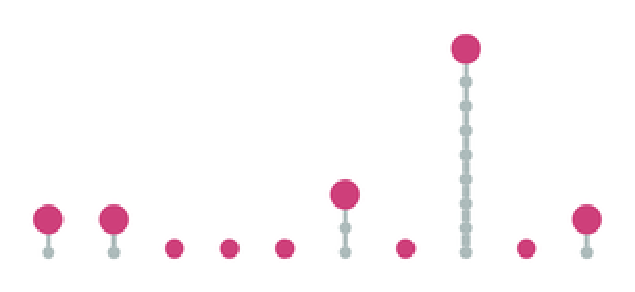
\includegraphics[scale=.25]{recAft.pdf}$
\end{lstlisting}

\subsubsection{Deargument and Program Induction}
In some sense the problem we are trying to address with the deargument transformation is the program induction problem itself.  We can view the values for each variable as data generated by some process we would like to identify i.e. there is some sort of common computation between variable values that we would like to represent as a program.  In the case of the noisy-number transformation we can view the generation of values for a single variable as coming from the same process, here we restrict the program representing this process to a Gaussian.  Similiary, in the case of the recursive transformation we can view the generation of values for a single variable as coming from a the same process, but we restrict the program representing this process to be the function being deargumented.  In the case of the same variable transformation we can view the generation of values for multiple variables as coming from the same process and we implicitly use the program for one variable as the generating process for the other.  It seems natural to ask whether we could reformulate the deargument transformation as recursive calls to the Bayesian program merging procedure in an attempt to find programs for generating the values of the variables.  One can think of this as recursively squeezing out the randomness in the data where the abstractions created by inverse-inlining create a separation between the ``structured'' parts of the data (the fixed common sub-expressions) and the random parts of the data (the variables in the expression patterns).  As an abstraction is applied one gets more data for the random parts and could conceivably attempt to learn a program to generate this data i.e. separate out even more structure.
\section{Experiments}
\subsection{Flower}
Here we used the following program to generate ten instances of flower that have alternating colors.  
\begin{lstlisting}
(define (flower shade)
  (lazy-list->all-list
   (N (data (color (gaussian 30 25)) (size .3))
      (N (data (color shade) (size .3)))
      (N (data (color shade) (size .3)))
      (N (data (color shade) (size .3))))))

(define flowers (repeat 10 (lambda () (flower (if (flip) 120 225)))))
\end{lstlisting}
An expression for these ten flowers was created using data incorporation and this expression was compressed into the program below using a beam width of 1 and depth of 30 for the beam search.
\begin{lstlisting}
(program
    ((abstraction F2 (V5) (data (color V5) (size 0.3)))
      (abstraction F1 (V2)
        ((lambda (V3)
           ((lambda (V1)
              ((lambda (V4)
                 (lambda ()
                   (N (F2 V1) (N (F2 V2)) (N (F2 V3))
                     (N (F2 V4)))))
                V3))
             35.8))
          V2)))
    (lambda ()
      ((uniform-draw
         (list (F1 220.0) (F1 257.0) (F1 117.0) (F1 226.0)
           (F1 250.0) (F1 110.0) (F1 237.0) (F1 120.0)
           (F1 133.0) (F1 146.0))))))
\end{lstlisting}

\section{Discussion}
We presented an approach to pattern recognition called Bayesian program merging.  The main ideas were to rerepresent data as a program and then frame pattern recognition as finding repeated computation in the program.   Finding repeated computation was performed through program transformations merged the structure of a program.  The sequences of transformations made while searching were guided using the posterior of the program.  

\subsection{Noisy Data Constructors}
We also allow for randomness in the data type constructors, which can lead to more compact representations of patterns in the presence of noise, which we will illustrate later.

It is worth noting the random nature of the color constructor.  Randomness in data constructors can potentially allow for compact representations of patterns in the presence of noise.  To get a sense of this idea look at figure \ref{noiseCons}. 
\begin{figure}[h]
\begin{center}
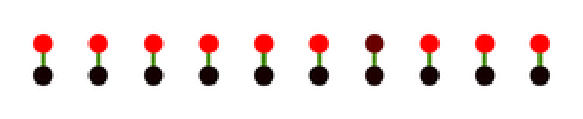
\includegraphics[scale=.60]{noisyConstructor.pdf}
\end{center}
\label{fig:noiseCons}
\caption{Some trees.}
\end{figure}
Without a noisy data constructor (i.e. if color were defined as \texttt{(define (color x) (node x))} we might create the following generative model:
\begin{lstlisting}
(multinomial-draw
 (node (data (color (gaussian 20 25)) (size .5)) (node (data (node 255) (size .5))))
 (node (data (node 20) (size .5)) (node (data (node 105) (size .5)))))
\end{lstlisting}
Which seems like a big penalty as far as model representation size goes since the probability of drawing the darker colored object may be incredibly small.  By having a noisy constructor we can model the data more compactly as simply 
\begin{lstlisting}
(node (data (color (gaussian 20 25)) (size .5)) (node (data (node 255) (size .5))))
\end{lstlisting}
This example only hints at the benefits of using probabilistic data constructors and probabilistic programs in general with respect to representation, but understanding the full implications of such a design decision and its impact on program induction are left as future work.

\subsection{Future Directions}

Future directions include using search strategies more sophisticated than beam search and looking at better ways to compute the likelihood.  Another open question is what happens when the data incorporation step is not so easy and training data is not directly computed in terms of some algebraic data type and whether one can impose some semblance of structure on unstructured data in order to use these methods for learning.  There are many other barriers to overcome before probabilistic program induction can compete with state-of-the-art machine learning algorithms on real world problems, but the increased potential for capturing rich patterns and less dependence on human engineering make research in the subject a worthy pursuit.
\bibliographystyle{plain}
\bibliography{myBib}
\end{document}
